\section{Exact inference (tree-structured BN) }
\subsection{Variable elimination}
- Given a BN and query $P(X|E=e)$\\
- Choose an ordering of $X_1, ..., X_n$ \textbf{Eliminate variables from the outside in!}\\
- Set up initial factors: $f_i=P(X_i|Pa_i)$\\
- For $i=1:n, X_i \notin {X, E}$\\
$\quad$ - Collect and multiply all factors $f$ that include $X_i$\\
$\quad$ - Generate new factor by marginalizing out $X_i$:
        ${g_X}_i = \sum_{x_i}\prod_j f_j$\\
$\quad$ - Add g to set of factors\\
- Renormalize $P(x,e)$ to get $P(x|e)$

\textbf{Variable elimination for polytrees:}\\
- Pick a root, (avoiding $X$ and $E$)\\
- Orient edges towards root\\
- Eliminate variables according to topological order


\subsection{Avoiding recomputation: factor graphs}
FG for a BN is a bipartite graph consisting of variables (circles) and factors (rectangles). \textbf{It is not a unique representation.}\\
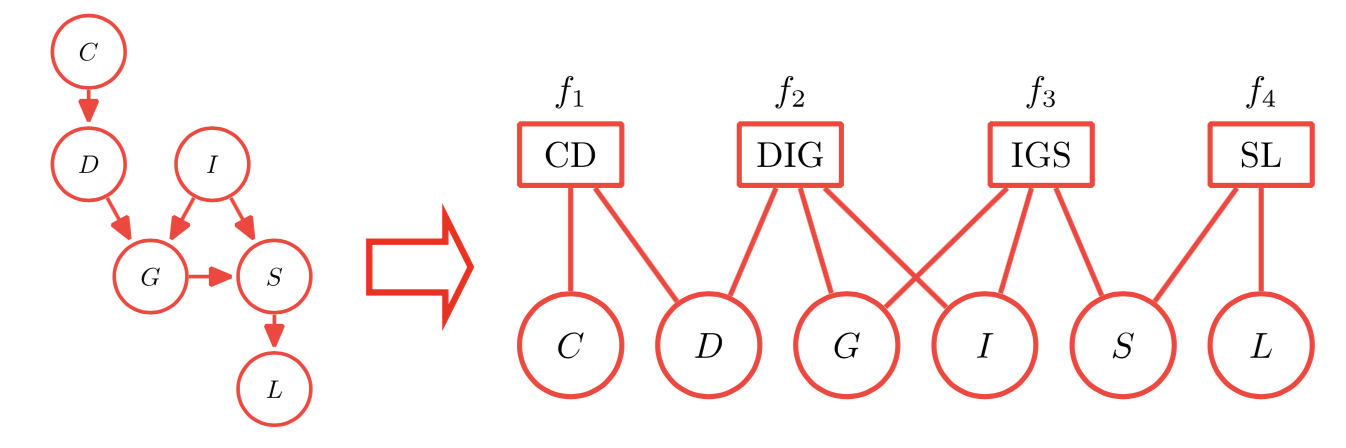
\includegraphics[scale=0.25]{images/factor_graph.png}
\subsubsection{Sum-product/Belief Propagation (BP) Algorithm:}
- Initialize all messages as uniform distribution\\
- Until converged to:\\
$\quad$ - Pick a root in the factor graph and reorient the edges towards this root.\\
$\quad$ -  Update messages according to this ordering. Do passes from leaves to root and from root to leaves.\\
- If a leaf node is a variable node: 
$\mu_{x\rightarrow f}(x)=1$
- If a leaf node is a factor node:
$\mu_{f \rightarrow x}(x)=f(x)$
- Messages from node $v$ to factor $u$:\\
    $\mu_{v\rightarrow u}(x_v) = \prod_{u'\in N(v)\setminus \{u\}}\mu_{u'\rightarrow v(x_v)}$\\
- Messages from factor $u$ to node $v$:\\
    $\mu_{u\rightarrow v}(x_v) = \sum_{x_u\sim x_v}f_u(x_u) \prod_{v'\in N(u)\setminus \{v\}}\mu_{v'\rightarrow u(x_v')}$
    % https://tex.stackexchange.com/questions/9363/how-does-one-insert-a-backslash-or-a-tilde-into-latex
$\quad$ -  Break once all messages change by $\leq \epsilon$

\textbf{Hope:} after convergence, we have:\\
$P(X_v=x_v)=\frac{1}{Z}\prod_{u \in N(v)}\mu_{u\rightarrow v}(x_v)$\\
$P(\overrightarrow{X_u}=\overrightarrow{x_u})=\frac{1}{Z} f_u(\overrightarrow{x_u})\prod_{v\in N(u)}\mu_{v\rightarrow u}(x_v)$

\textbf{If we have a polytree Bayesian network}:\\
- Choose one node as root\\
- Send messages from leaves to root and from root to leaves\\
